\documentclass[]{IEEEphot}
\jvol{1}
\jnum{4}
\jmonth{Marth}
\pubyear{2012}
\usepackage{graphicx}
\usepackage{fontspec}
\XeTeXlinebreaklocale "zh" %针对中文进行断行
\setmainfont{WenQuanYi Zen Hei} %设置默认的字体
\linespread{1.2}

\begin{document}
\title{数字图像处理实验四\\实验报告}
\author{040920112 戴一冕}
\maketitle
\markboth{数字图像处理}{实验四实验报告}
\begin{abstract}
运用Sobel,Laplacian,Roberts算子分别对图像进行锐化操作 
\end{abstract}
\begin{IEEEkeywords}
Sobel,Laplacian,Roberts,锐化
\end{IEEEkeywords}
\section{实验目的}
通过上机实验的手段巩固课堂上所学的关于图像锐化的相关知识,自己编写Sobel,Laplacian,Roberts算子对图像进行锐化的函数,感受不同的图像处理方法对最终图像效果的影响。
\section{实验内容}
\subsection{方法技术介绍}
锐化处理的主要目的是突出图像中的细节或者增强被模糊了的细节,这种模糊不是由错误操作造成的,就是特殊图像获取方法的固有影响。从前面几个实验中可以知道,在空域用像素邻域平均法可以使图像变模糊,因为均值处理与积分类似,从逻辑角度可以断定,锐化处理可以用空间微分来完成。下文将分别讨论Sobel算子、Laplacian算子和Roberts算子这三个微分锐化算子。
\subsubsection{Sobel算子}
在图像处理中,一阶微分是通过梯度法实现的。对于函数$f(x,y)$在其坐标$(x,y)$上的梯度是通过如下二维列向量定义的:
\begin{equation}
	\nabla f =
	\left[
		\begin{array}{c}
			G_x\\
			G_y
		\end{array}
	\right]
	=
	\left[
		\begin{array}{c}
			\frac{\partial f}{\partial x}\\
			\frac{\partial f}{\partial y}
		\end{array}
	\right]
	\label{eql}
\end{equation}
这个向量的模值由下式给出:
\begin{eqnarray}
	\nabla f & = & mag(\nabla \bf f)\\
		  {} & = & [G_x^2+G_y^2]^{\frac{1}{2}}\\
	   {} & = & [(\frac{\partial f}{\partial x})^2+(\frac{\partial f}{\partial y})^2]^{\frac{1}{2}}
\end{eqnarray}
Sobel算子属于一阶微分处理,对于一元函数$f(x)$,表达一阶微分的定义是一个差值:
\begin{equation}
	\frac{\partial f}{\partial x}=f(x+1)-f(x)
	\label{eql}
\end{equation}
对于水平和垂直两个方向,相应就有水平Sobel和垂直Sobel两个模板。
\[
	d_x=\left[
		\begin{array}{lcr}
			-1 & -2 & -1 \\
			 0 & 0 & 0 \\
			 1 & 2 & 1
		\end{array}
	\right]
	(水平Sobel)\indent
	d_y=\left[
		\begin{array}{lcr}
			-1 & 0 & 1 \\
			-2 & 0 & 2 \\
			-1 & 0 & 1
		\end{array}
	\right]
	(垂直Sobel)
\]
综合考虑水平和垂直两个方向,则采用$\sqrt{d_x^2+d_y^2}$来生成图像,也就是$(4)$式。
\subsubsection{Laplacian算子}
下式用差分定义$x$方向上的二阶微分:
\begin{equation}
	\frac{\partial^2f}{\partial x^2}=f(x+1,y)+f(x-1,y)-2f(x,y)
	\label{eql}
\end{equation}
相应的,$y$方向上的二阶微分则为:
\begin{equation}
	\frac{\partial^2f}{\partial y^2}=f(x,y+1)+f(x,y-1)-2f(x,y)
	\label{eql}
\end{equation}
二维拉普拉斯数字实现可由这两个分量相加得到:
\begin{equation}
	\nabla^2f=[f(x+1,y)+f(x-1,y)+f(x,y+1)+f(x,y-1)]-4f(x,y)
	\label{eql}
\end{equation}
于是,Laplacian的算子形式便为:
\[
	\left[
		\begin{array}{lcr}
			0 & -1 & 0 \\
		-1 & 4 & -1 \\
			0 & -1 & 0 
		\end{array}
	\right]
\]
带对角线的Laplacian算子为:
\[
	\left[
		\begin{array}{lcr}
			-1 & -1 & -1 \\
			-1 &  8 & -1 \\
			-1 & -1 & -1
		\end{array}
	\right]
\]
假设有一个灰度值均匀变化的斜坡,其上的一阶微分值都不是零,但是二阶微分只有在斜坡的起始处和终点处才不为零。在图像中,边缘类似于这种过渡,进而可以得出一阶微分产生较粗的边缘,而二阶微分则细的多。可见二阶微分对细节的处理好于一阶微分。但考虑到孤立噪声点的情况,在该噪声点及其周围,二阶微分比一阶反应要强的多,也就是说二阶微分对噪声敏感。
\subsubsection{Roberts算子}
当对整幅图像进行$(4)$式的计算时,计算量很大,因此在实际操作中常用绝对值代替平方与开放运算近似求梯度的模值:
\begin{equation}
	\nabla f\approx |G_x|+|G_y|\\
	\label{eql}
\end{equation}
Roberts于1965年提出两种定义使用了交叉差分的算法:
\begin{eqnarray}
	G_x=f(x+1,y+1)-f(x,y)\\
	G_y=f(x+1,y)-f(x,y+1)
\end{eqnarray} 从而可以得到梯度的近似算法: 
\begin{equation} 
	\nabla f\approx |f(x+1,y+1)-f(x,y)|+|f(x+1,y)-f(x,y+1)| \label{eql}
\end{equation}
\subsection{实验步骤}
\subsubsection{步骤1}
编写好Sobel,Laplacian,Roberts算子的相关函数,整理成一个模块,以便于后面的实验。
\subsubsection{步骤2}
读入cameraman.jpg图像文件,分别采用垂直方向的Sobel算子,Laplacian算子和$\sqrt{d_x^2+d_y^2}$的Sobel算子对原图进行锐化处理。
\subsubsection{步骤3}
\begin{enumerate}
	\item 读入skeleton.jpg文件,用带对角线的Laplacian算子对其处理。
	\item 将1)的结果叠加到原始图像上。可看出噪声增强了(Laplacian算子对噪声敏感),应设法降低。
	\item 获取Sobel图像并进行$5\times5$邻域平均,以减少噪声。
	\item 获取2)和3)相乘图像,噪声得以减少。
	\item 将4)结果叠加到原始图像上。
	\item 最后对5)的图像做幂指数为0.2的幂次变换
\end{enumerate}
\subsubsection{步骤4}
编写Roberts梯度锐化函数,对cell.jpg进行图像锐化,锐化图像的形成以下式为准:
\begin{equation}
	g(x,y)=
	\left\{
		\begin{array}{lr}
			L_G, & G[f(x,y)]\geq T\\
			L_B, & otherwise
		\end{array}
	\right.
\end{equation}
$L_G=255,L_B=0$,适当选择门限T。
\section{实验结果与分析}
\subsection{实验环境介绍}
本实验采用Python 2.7.2及其Numpy,Scipy,PIL,matplotlib,以及我自己编写的PyDIP模块,同时有用Matlab再实验了一次以用来对照。
Numpy,Scipy,PIL,matplotlib均可以从其官网上方便的下到,而PyDIP我把它放到了github上,可以在PyDSP这个项目下直接找到,也可以从PyEE的modules文件夹内找到。后续的一些函数文档,我会陆续放在D\&L上。
\subsection{结果分析}
\subsubsection{步骤1}
所有的函数均写在PyDIP模块内,是按照最基本的定义来写的,没有做更多的优化。
\subsubsection{步骤2}
步骤2的结果如图所示,与原图像对照,三种处理方法均提取出了轮廓。
\begin{figure}[h]
	\centering
	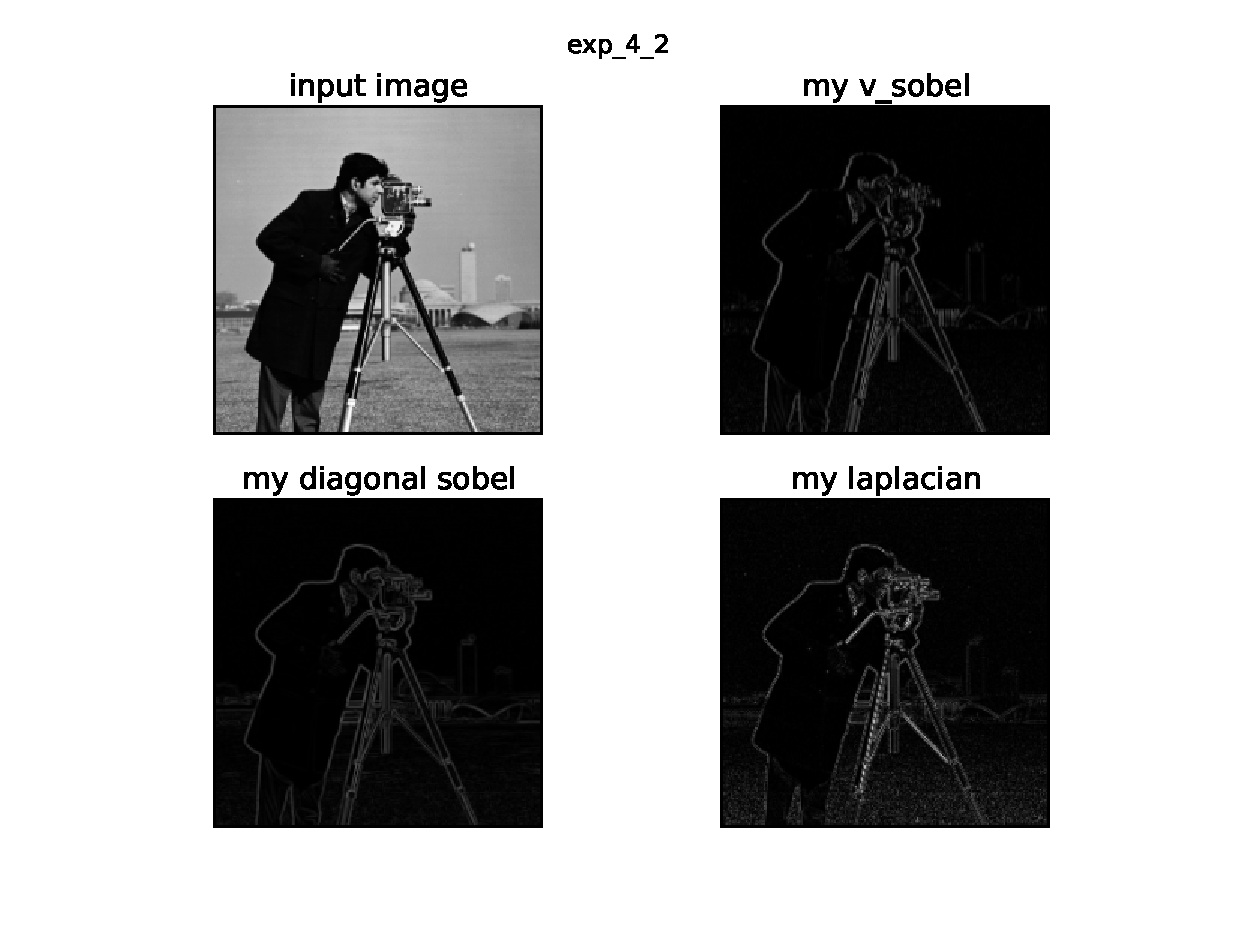
\includegraphics[width=20pc]{exp_4_2.eps}
	\caption{(a)步骤2结果图}
	\label{fig_env1}
\end{figure}
垂直方向的Sobel算子在摄影师肩膀那一段的轮廓没有提取出来,而对角线的Sobel和Laplacian均提取出来了,那是因为后两者均考虑了水平和垂直两个方向,而垂直Sobel没有考虑,所以也就没有提取出水平方向变化的信息。
在上文中讲到,Laplacian算子属于二阶微分,而Sobel是一阶微分,二阶微分相比一阶微分所处理的图像,轮廓线更加细,但由于这张图像中在人物的轮廓周边灰度变化很快,所以Laplacian算子没有体现出这一点来。
\subsubsection{步骤3}
\begin{figure}[h]
	\centering
	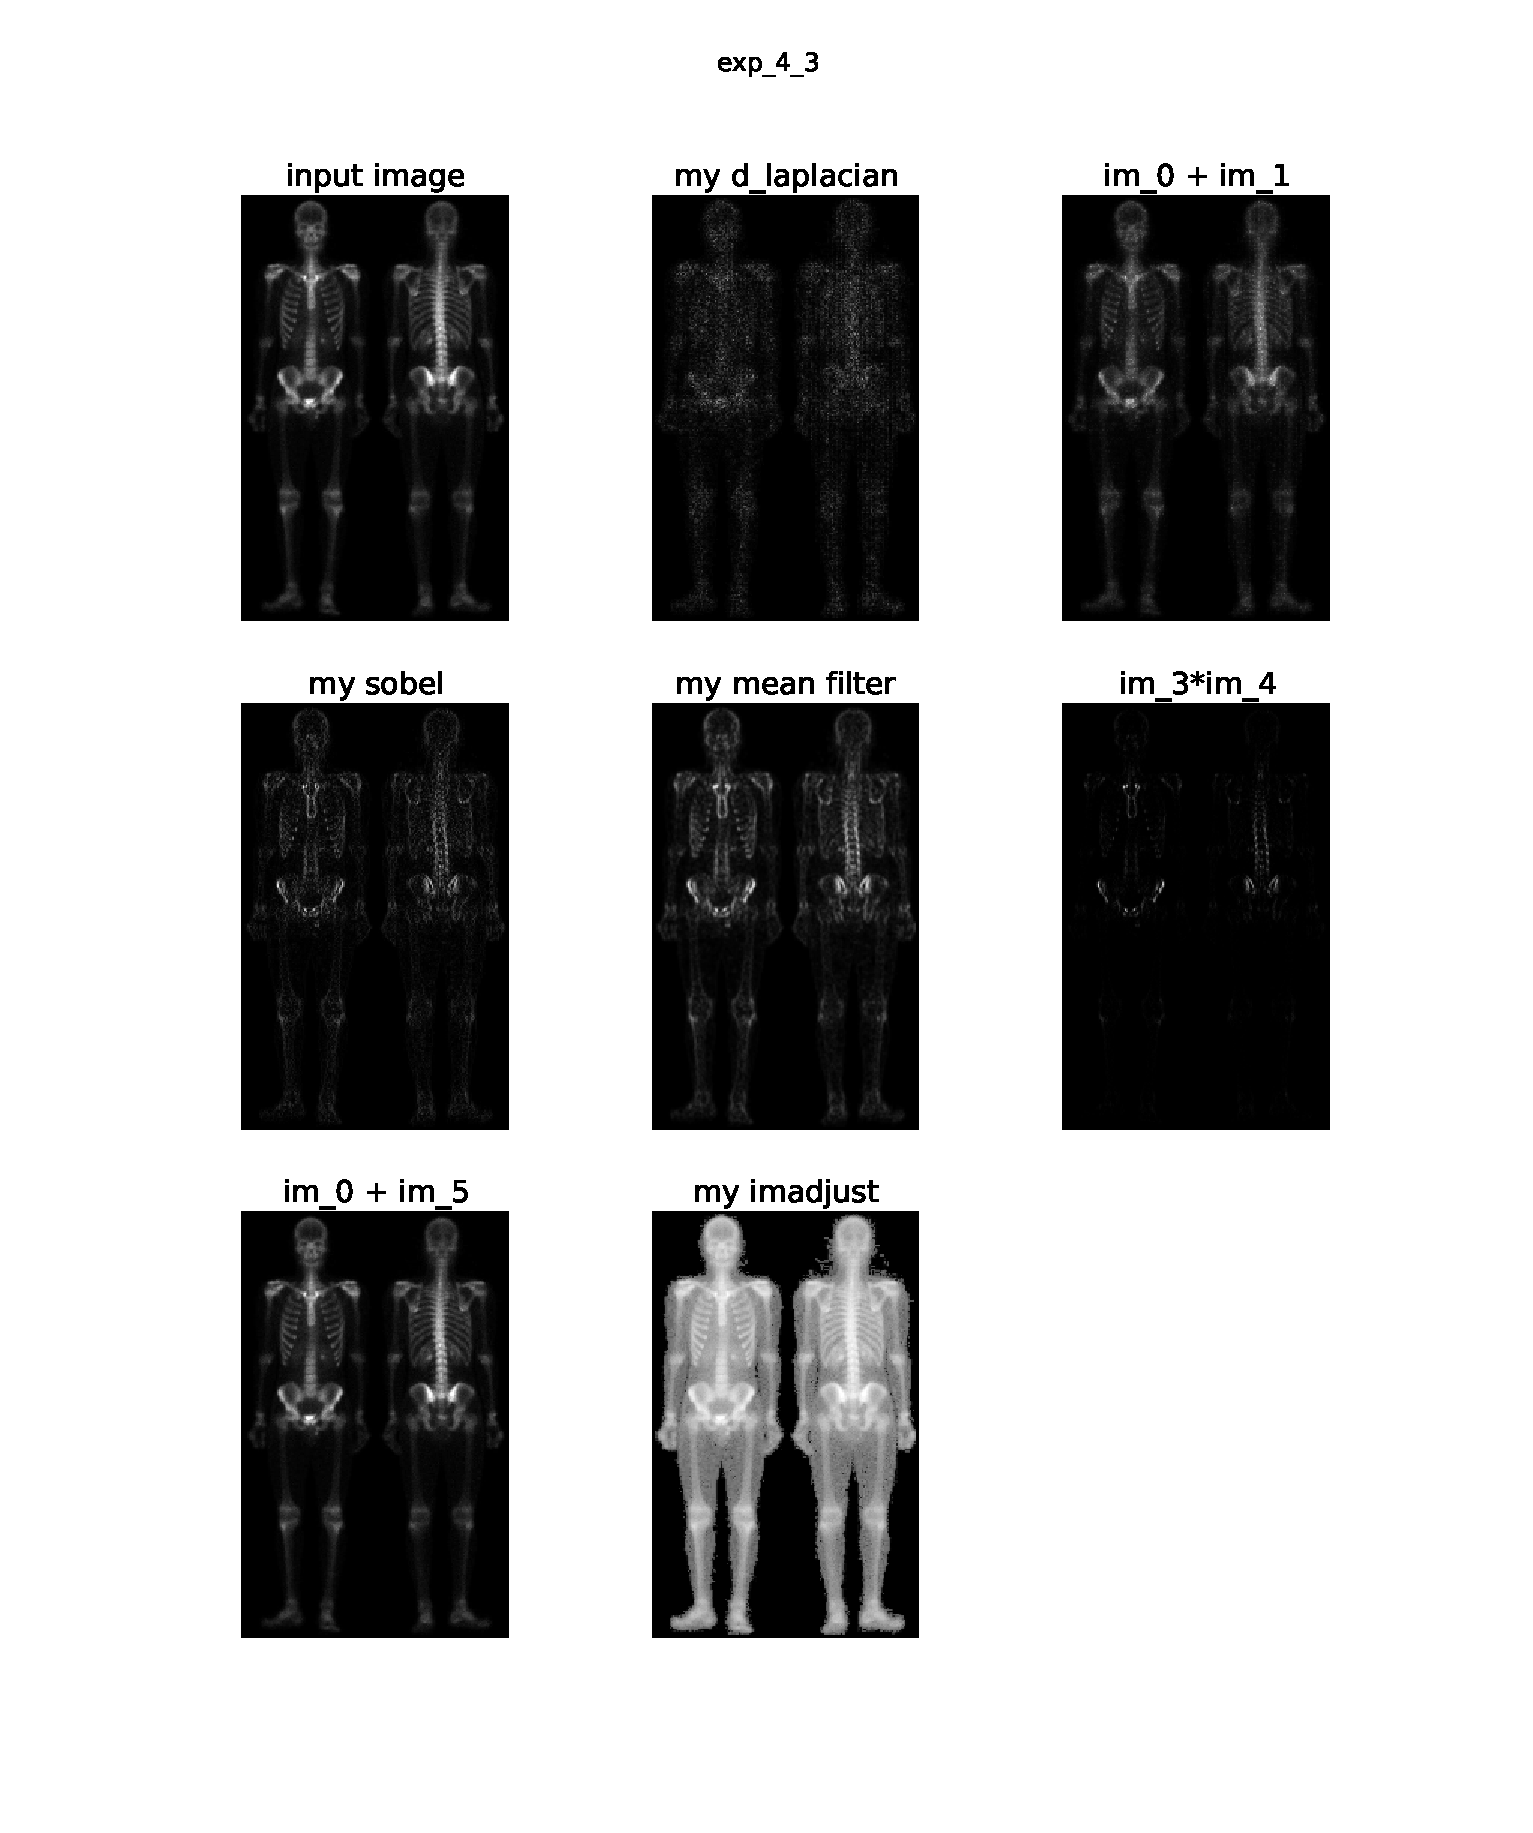
\includegraphics[width=20pc]{exp_4_3.eps}
	\caption{(b) 步骤3结果图}
	\label{fig_env1}
\end{figure}
对角线的Laplacian对原图进行处理后效果并不好,都是一些散点,这是由于二阶微分对噪声敏感造成的,在将其叠加到原图上与原图对比,可以看出变模糊了。使用Sobel算子对原图进行处理得到的图像效果好于用Laplacian的结果,进行均值滤波后更加清晰。
对于将2)和3)的图像相乘,我猜想原理应该跟离散数学里的与运算一样,对于某一个点的灰度值,我很难判断究竟是噪声还是真实值,对于两种处理的效果相乘,如果一个为0,一个有较大的灰度值,即可判断这个点是噪声噪声的,相乘的结果也就消除了噪声。故而,相乘解雇结果的图像变得更为清晰,但是灰度值普遍偏小,图像有点暗。
叠加到原图上后,加强了目标区域的灰度值,是的图像更为清晰。而进行幂次运算,能够让窄带的灰度值小的区间分布在一个较大的灰度值区间内,目标也就更为明亮。
\subsubsection{步骤4}
这里需要先提以下matplotlib的问题,用imshow显示的读入的灰度图片与实际灰度图片有偏差,cell的原图是比较灰蒙蒙的,但是用imshow显示出来的就像预先坐过了灰度拉伸等的处理,显得很清楚,但这就给我后期Roberts变换带来了不便,效果与matlab上做的有点偏差。
\begin{figure}[h]
	\centering
	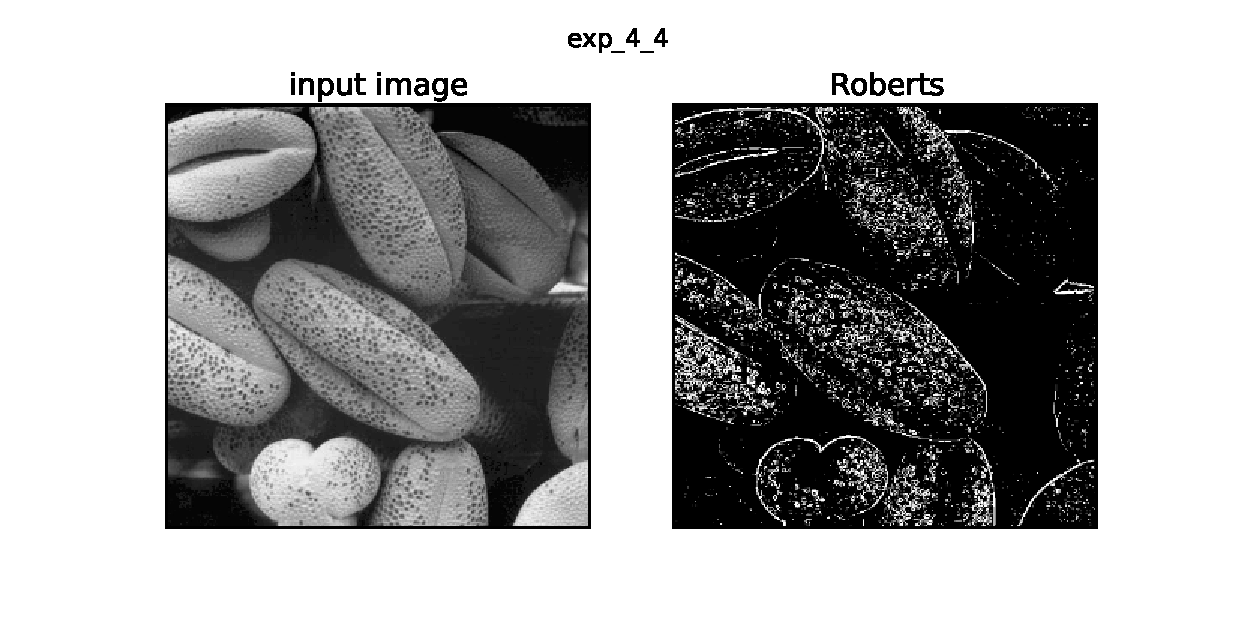
\includegraphics[width=20pc]{exp_4_4.eps}
	\caption{(c) 步骤四结果图}
	\label{fig_env1}
\end{figure}
我理解的Roberts算子是Sobel算子的简化,相对于Sobel算子,Roberts算子的运算量大大简化,上图是我选取了门限$T=10$的时候的情形。可以看得出,Roberts算子也能不错的提取出轮廓信息,细胞上的一些小斑点也能体现出来。
\section{心得体会}
四个实验均做完了。\\
感谢这次实验,让我萌生了在github上建了一个名为PyEE的open source的项目的念头,并且已经付之于行动了。在这个过程中,运用Python,结合课堂上的内容,我写了PyDIP的模块。不仅增强了对数字图像处理的了解,也锻炼了编程能力,可谓一举两得。
还有,在这次实验中我用到的Numpy、Scipy、matplotlib和PIL,这四个类库的中文资料很很稀少,为了完成实验我阅读了不少的英文资料,锻炼了阅读文档和信息检索的能力。
至此,我体会到知行合一才是学习知识的王道,以前那些专业课如果也能开设这样的上机软实验就好了。
\section{附件}
随实验报告的文件夹内有Python和Matlab的源程序,由于这是PyEE的一部分,最新的程序会放在github的PyEE项目上。本实验中涉及的函数在PyDSP项目内。
\end{document}
